\documentclass[brazilian]{beamer}
\usetheme{CambridgeUS}
\usecolortheme{beaver}

% \usepackage[utf8]{inputenc}
\usepackage{babel}
\usepackage{ragged2e}
\apptocmd{\frame}{}{\justifying}{}

\usepackage{xcolor}
\definecolor{emerald}{rgb}{0.31, 0.78, 0.47}

\usepackage{caption}
\usepackage{hyperref}
\hypersetup{
    unicode=true,
    pdfstartview={FitV},
    pdfauthor={Nightwind},
    pdfkeywords={latex, dicas},
    colorlinks=true,
    linkcolor=black,
    citecolor=green,
    filecolor=cyan,
    urlcolor=magenta
}
\usepackage[nameinlink,capitalise]{cleveref}
\usepackage[style=abnt]{biblatex}
\addbibresource{references.bib}
\usepackage{csquotes}

\usepackage{tabularx}
\usepackage{array}
\newcolumntype{M}[1]{>{\raggedleft\arraybackslash}m{#1}}
\newcolumntype{O}[1]{>{\raggedright\arraybackslash}m{#1}}
\newcolumntype{C}[1]{>{\centering\arraybackslash}m{#1}}
\usepackage{multirow}

\usepackage{graphicx}
\usepackage{svg}

\usepackage{multicol}
\usepackage{fontspec}
\setsansfont{Syne}
\setmonofont{Space Mono}
\usefonttheme[onlymath]{serif}

\usepackage{mathtools}
\usepackage{mathrsfs}
\usepackage{xfrac}
\DeclareMathOperator{\sen}{sen}
\newcommand{\intd}[4]{\ensuremath{\int_{#1}^{#2}\left[#3\right]\,\mathsf{d}{#4}}}
\newcommand{\edp}[3][]{\ensuremath{\frac{\partial^{#1}\left[#2\right]}{\partial{#3}^{#1}}}}

\usepackage{listings}
\definecolor{asparagus}{rgb}{0.53, 0.66, 0.42}
\definecolor{lavendergray}{rgb}{0.77, 0.76, 0.82}
\definecolor{pastelmagenta}{rgb}{0.96, 0.6, 0.76}
\definecolor{mistyrose}{rgb}{1.0, 0.89, 0.88}
\definecolor{packagecolor}{rgb}{1.0, 0.0, 0.16}
\definecolor{darkslateblue}{rgb}{0.28, 0.24, 0.55}
\definecolor{forestgreen}{rgb}{0.13, 0.55, 0.13}

\lstdefinestyle{myStyleLatex}{
    language=[LaTeX]TeX,
    backgroundcolor = \color{mistyrose},
    basicstyle = \ttfamily,
    breakatwhitespace = true,
    columns = fullflexible,
    breaklines = true,
    captionpos = a,
    commentstyle = {\footnotesize\color{asparagus}},
    escapeinside = {  {(*}  {*)}  },
    extendedchars = true,
    firstnumber = 1,
    frame = none,
    keepspaces = true,
    keywordstyle = {\bfseries\color{darkslateblue}},
    keywordstyle = [2]{\color{forestgreen}},
    keywordstyle = [3]{\itshape\color{packagecolor}},
    morekeywords = {maketitle,chapter,part, section, subsection, subsubsection, paragraph, subparagraph,familydefault,rmdefault,sfdefault,ttdefault,textsubscript,ttshape,colorbox,textcolor,definecolor,setlength,includegraphics,listoffigures,listoftables,endfirsthead,endhead,endfoot,endlastfoot,arraybackslash,newcolumntype,rowcolor,rowcolors,cellcolor,multirow,setmainfont,documentclass,mathcal,mathbb,mathfrak,mathscr,DeclareMathOperator,cref,autoref,lstdefinestyle,lstset,dfrac,sfrac,lstinline,lstinputlisting},
    morekeywords = [2]{default,arguments},
    morekeywords = [3]{document,command,definition, ambiente,book,report,article,exam, beamer,flushright,flushleft,center,figure,table,tabular,tabularx,longtable,article,book,exam,wrapfigure,equation,split,align,gather,multiline,lstlisting},
    numbers = left,
    numbersep = -1pt,
    numberstyle = \color{lavendergray},
    rulecolor = \color{magenta},
    showspaces = false,
    showstringspaces = false,
    showtabs = false,
    stepnumber = 1,
    stringstyle = \color{pastelmagenta},
    tabsize = 2
}

\usepackage[os=win]{menukeys}

\author{Nightwind}
\institute[CTISM]{Colégio Técnico Industrial de Santa Maria}
\logo{
\includegraphics[width=1cm]{../images/photo1.jpg}}
\date{\today}


\title{Utilizando o Overleaf}

\begin{document}

\frame{\titlepage}

\begin{frame}
    \frametitle{Sumário}
    \tableofcontents
\end{frame}

\section[Página Inicial]{Página Inicial do Overleaf}
\begin{frame}
    \frametitle{Homepage}
    \begin{figure}
        \centering
        \caption[HomePage]{Página Inicial do Overleaf.}
        \label{fig:homepageOverleaf}
        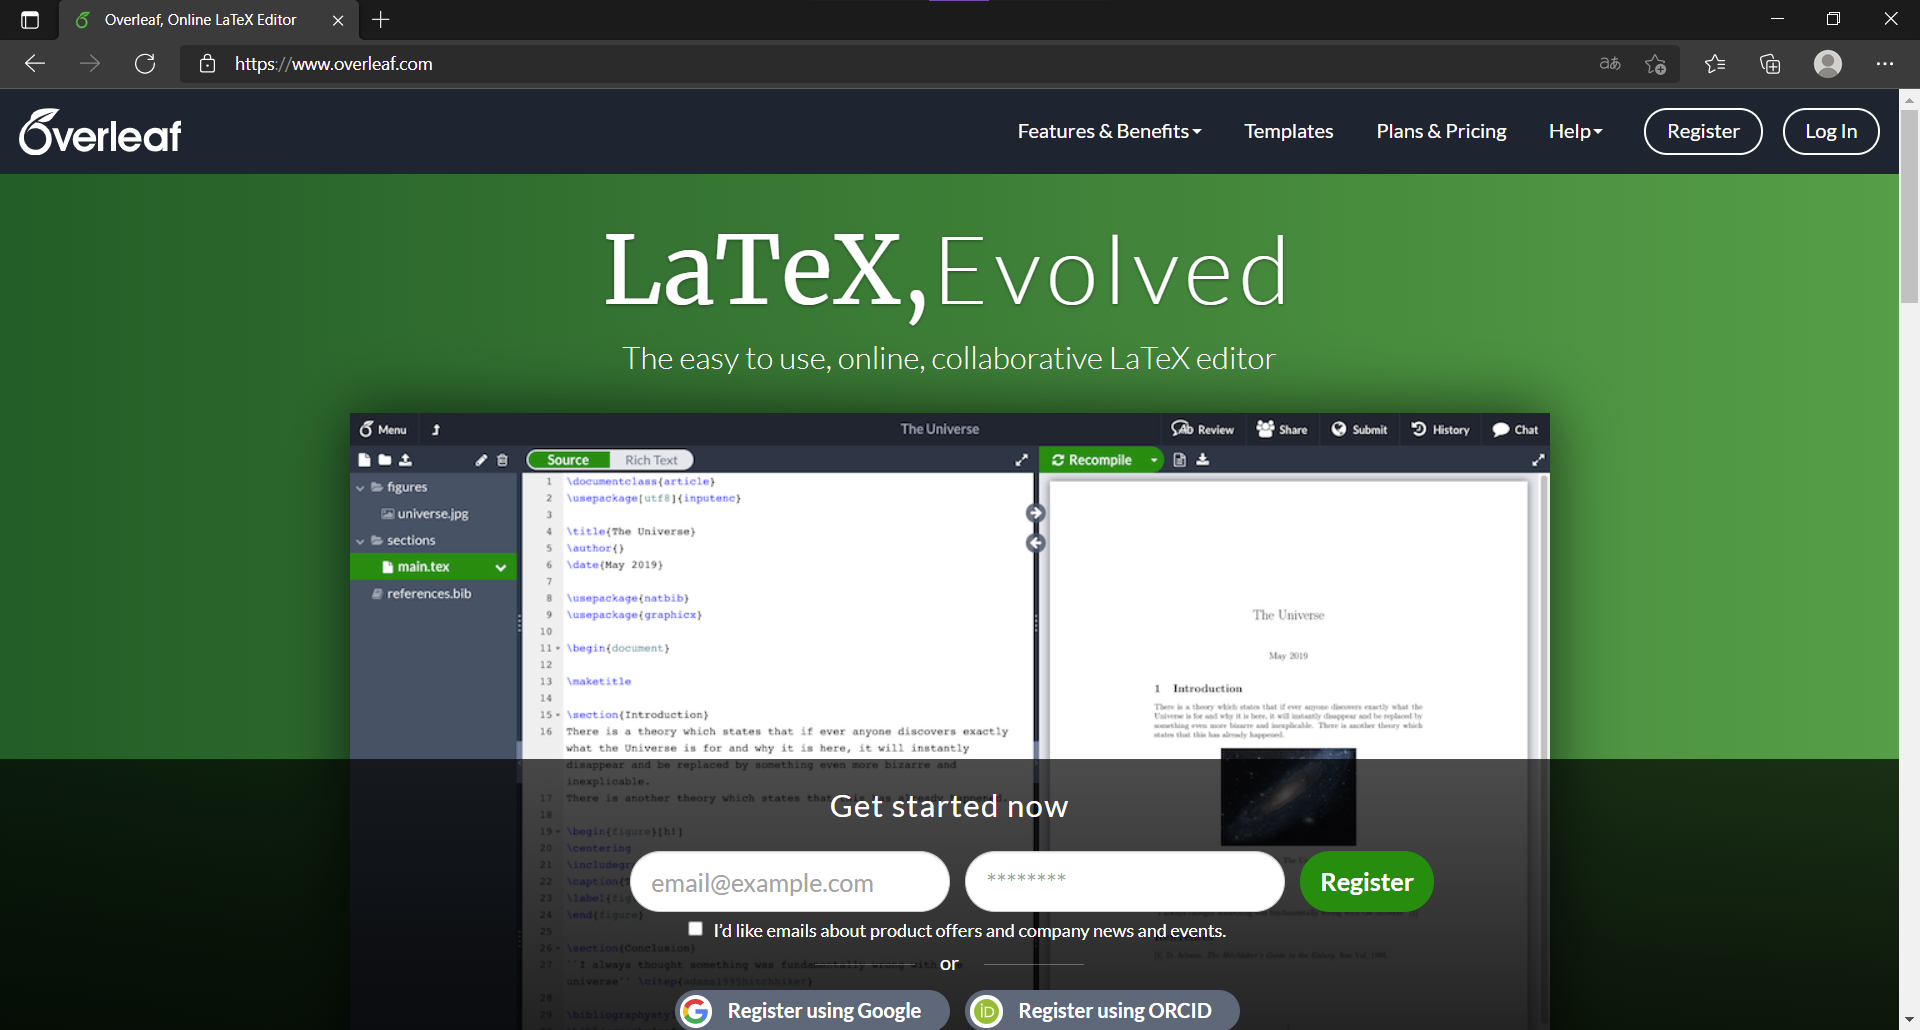
\includegraphics[width=0.8\textwidth]{../images/homepageOverleaf.png}
        \caption*{\footnotesize \url{https://www.overleaf.com/}}
    \end{figure}
\end{frame}

\begin{frame}
    \frametitle{Homepage}
    \begin{itemize}
        \item Vá em ``\textit{Register}'' caso ainda não tenha uma conta.
        \item Vá em ``\textit{Log In}'' caso já tenha uma conta.
        \item Coloque \textit{e-mail} e senha.
    \end{itemize}
\end{frame}

\section{Área do Usuário}
\begin{frame}
    \frametitle{Novo usuário}
    \begin{figure}
        \centering
        \caption{Área do novo usuário.}
        \label{fig:newUserOverleaf}
        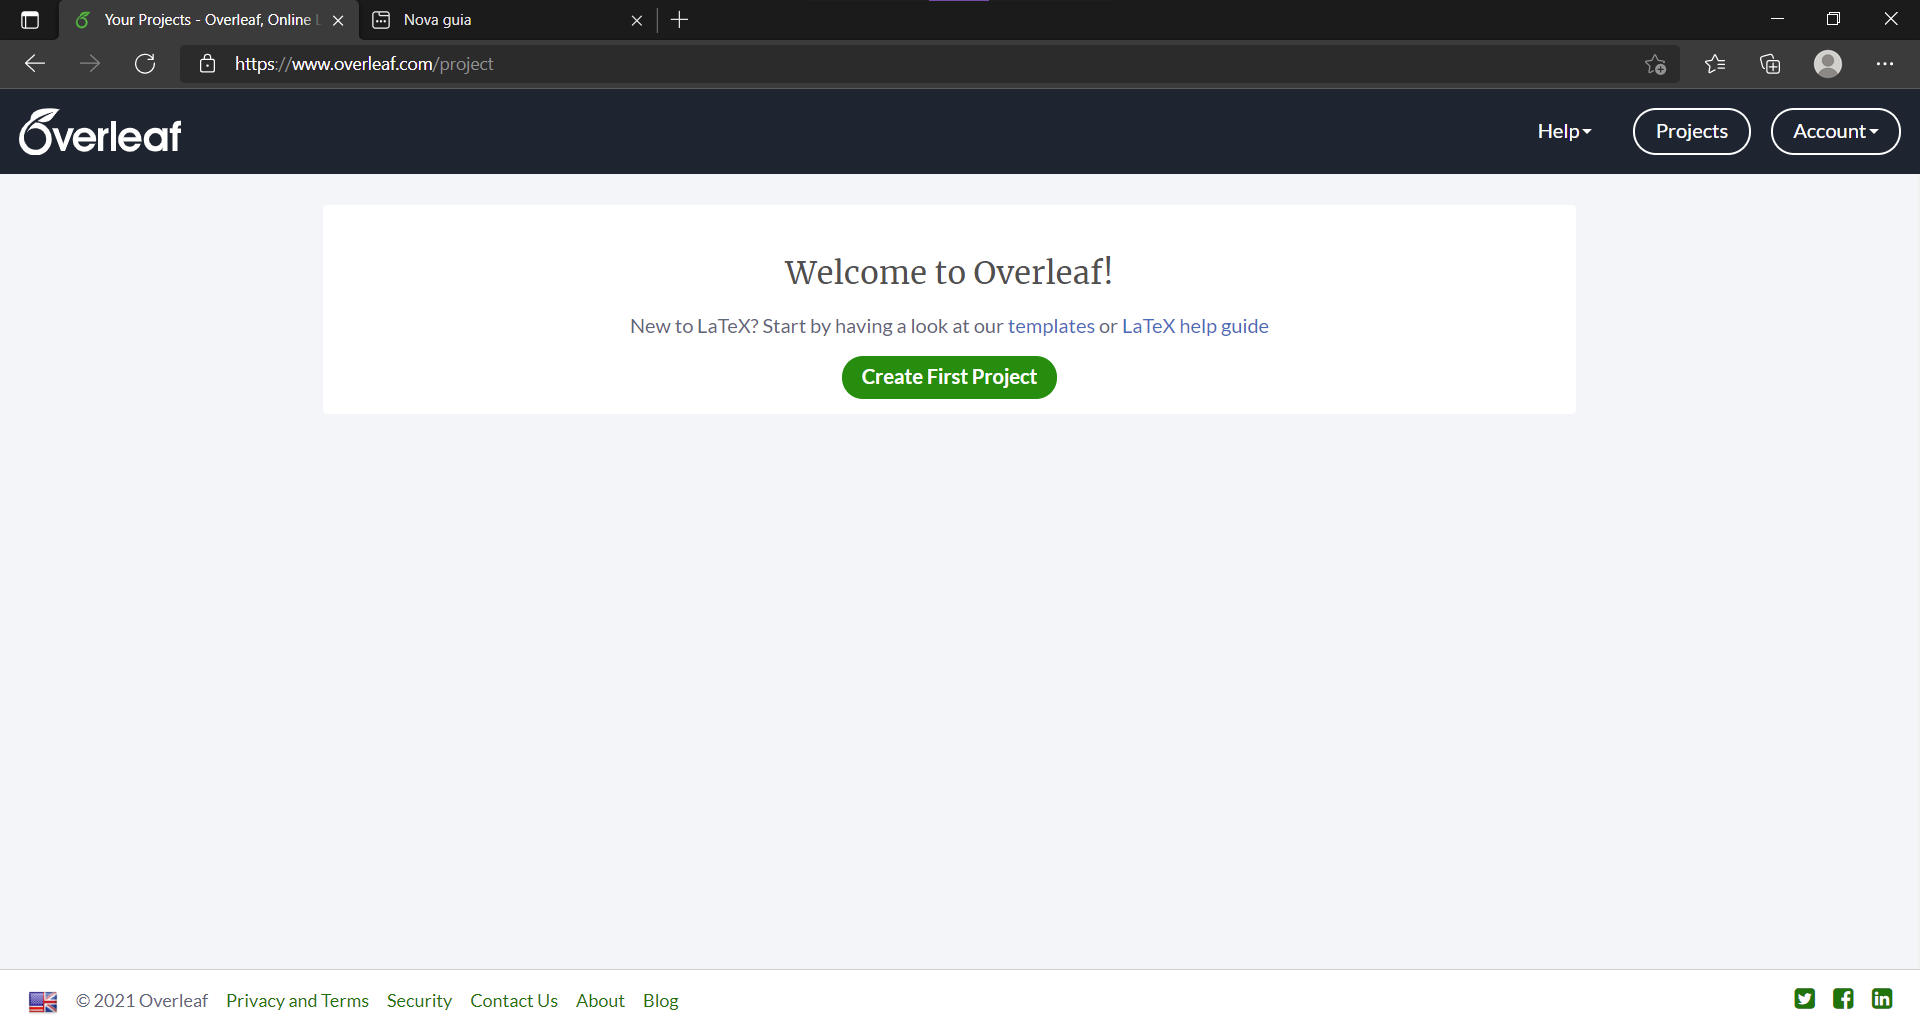
\includegraphics[width=0.8\textwidth]{../images/newUserOverleaf.png}
    \end{figure}
\end{frame}

\begin{frame}
    \frametitle{Primeiro Documento}
    \begin{columns}
        \begin{column}{0.5\textwidth}
            \begin{itemize}
                \item Para novos usuários, o \href{https://www.overleaf.com/}{Overleaf} recomenda visualizar os \href{https://www.overleaf.com/latex/templates}{Templates} e o \href{https://www.overleaf.com/learn}{Guia de \LaTeX}. Ambos são altamente recomendáveis.
                \item Para criar o primeiro projeto, clicar em ``\textit{Create First Project}''.
                \item Uma lista de opções aparecerá, como mostra a \autoref{fig:createANewProject}.
            \end{itemize}
        \end{column}
        \begin{column}{0.5\textwidth}
            \begin{figure}
                \centering
                \caption{Opções de Projeto.}
                \label{fig:createANewProject}
                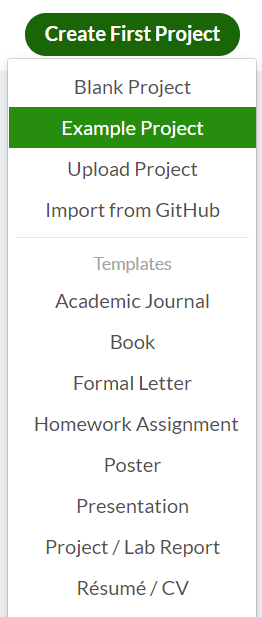
\includegraphics[width=0.3\textwidth]{../images/createANewProject.png}
            \end{figure}
        \end{column}
    \end{columns}
\end{frame}

\section{Novo documento}

\begin{frame}
    \frametitle{Novo documento}
    \begin{itemize}
        \item Para fins de ilustração, a opção escolhida foi ``\textit{Blank Project}''.
    \end{itemize}
    
    
\end{frame}

\begin{frame}
    \frametitle{Novo documento}
    \begin{figure}
        \centering
        \caption{Nomeando um novo documento.}
        \label{fig:nameOfProject}
        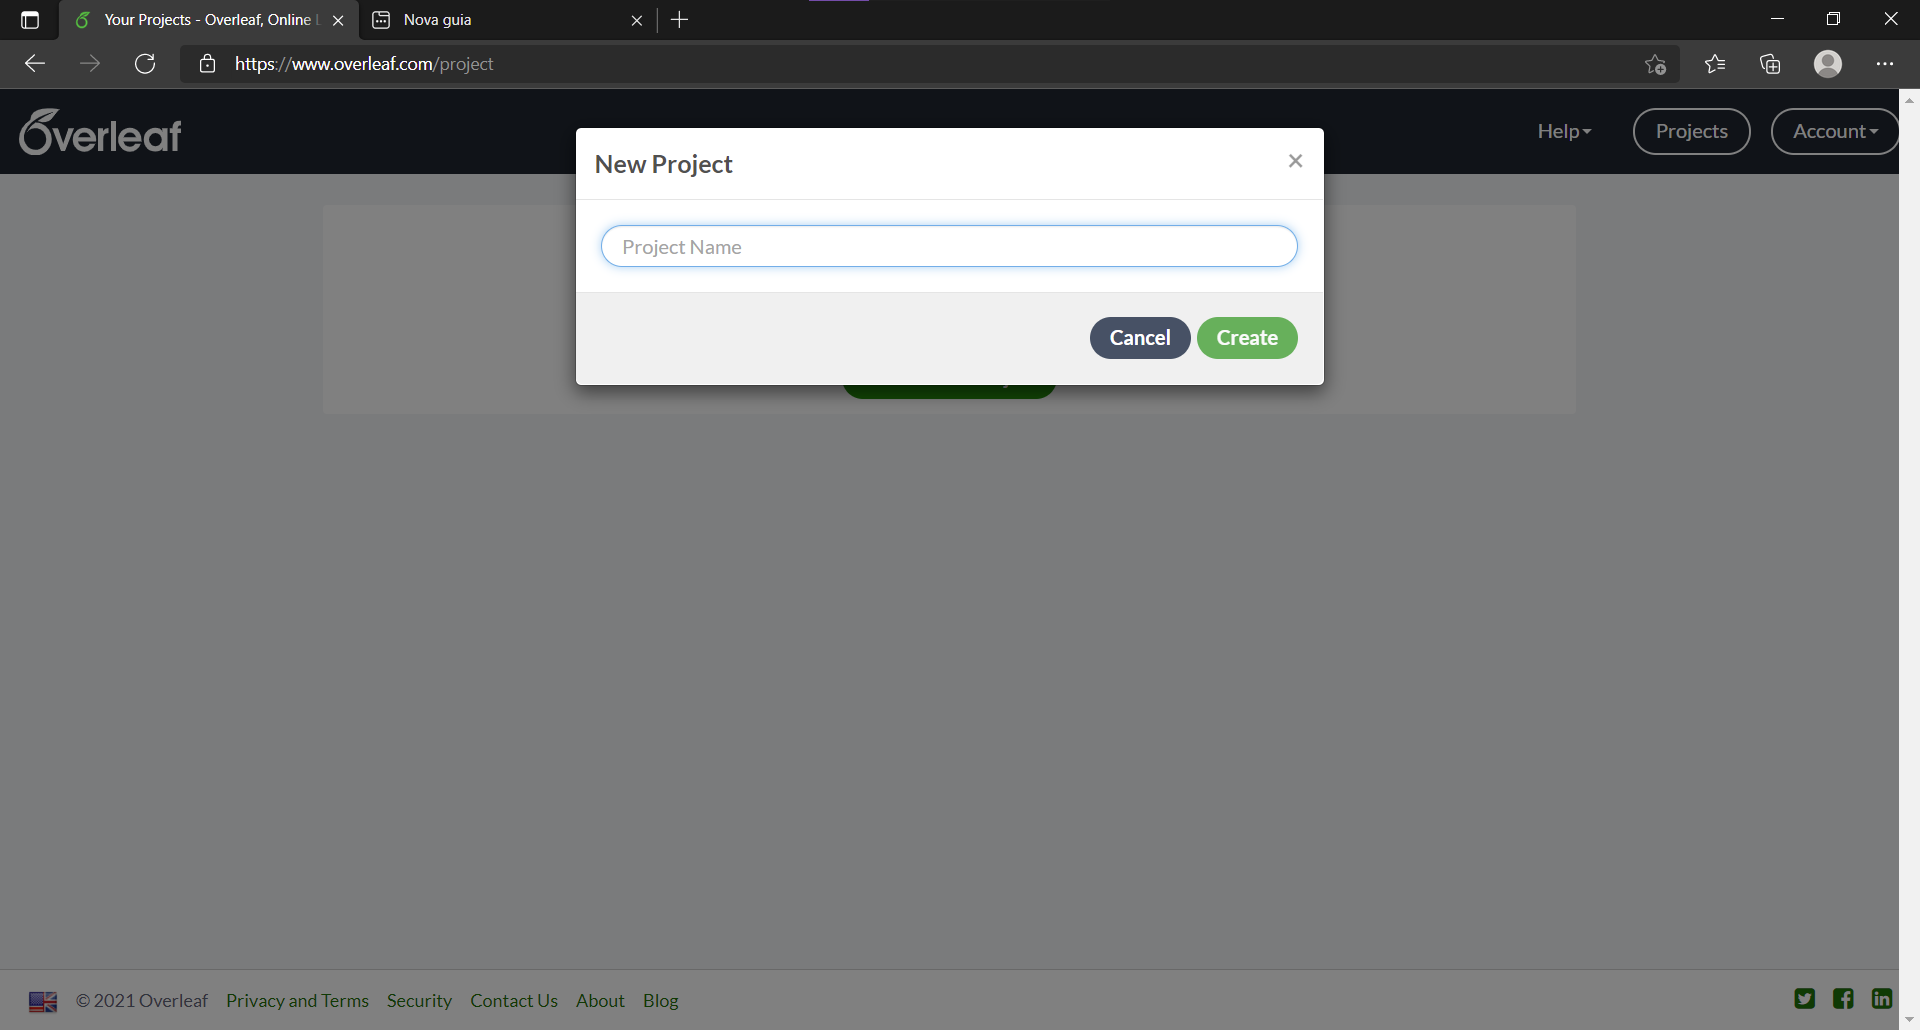
\includegraphics[width=0.8\textwidth]{../images/nameOfProject.png}
    \end{figure}
\end{frame}

\begin{frame}
    \frametitle{Novo documento}
    \begin{itemize}
        \item Depois de dar o nome da sua preferência, clique em ``\textit{Create}''.
    \end{itemize}
\end{frame}

\begin{frame}
    \frametitle{Novo documento}
    \begin{figure}
        \centering
        \caption{Documento em branco.}
        \label{fig:blankProject}
        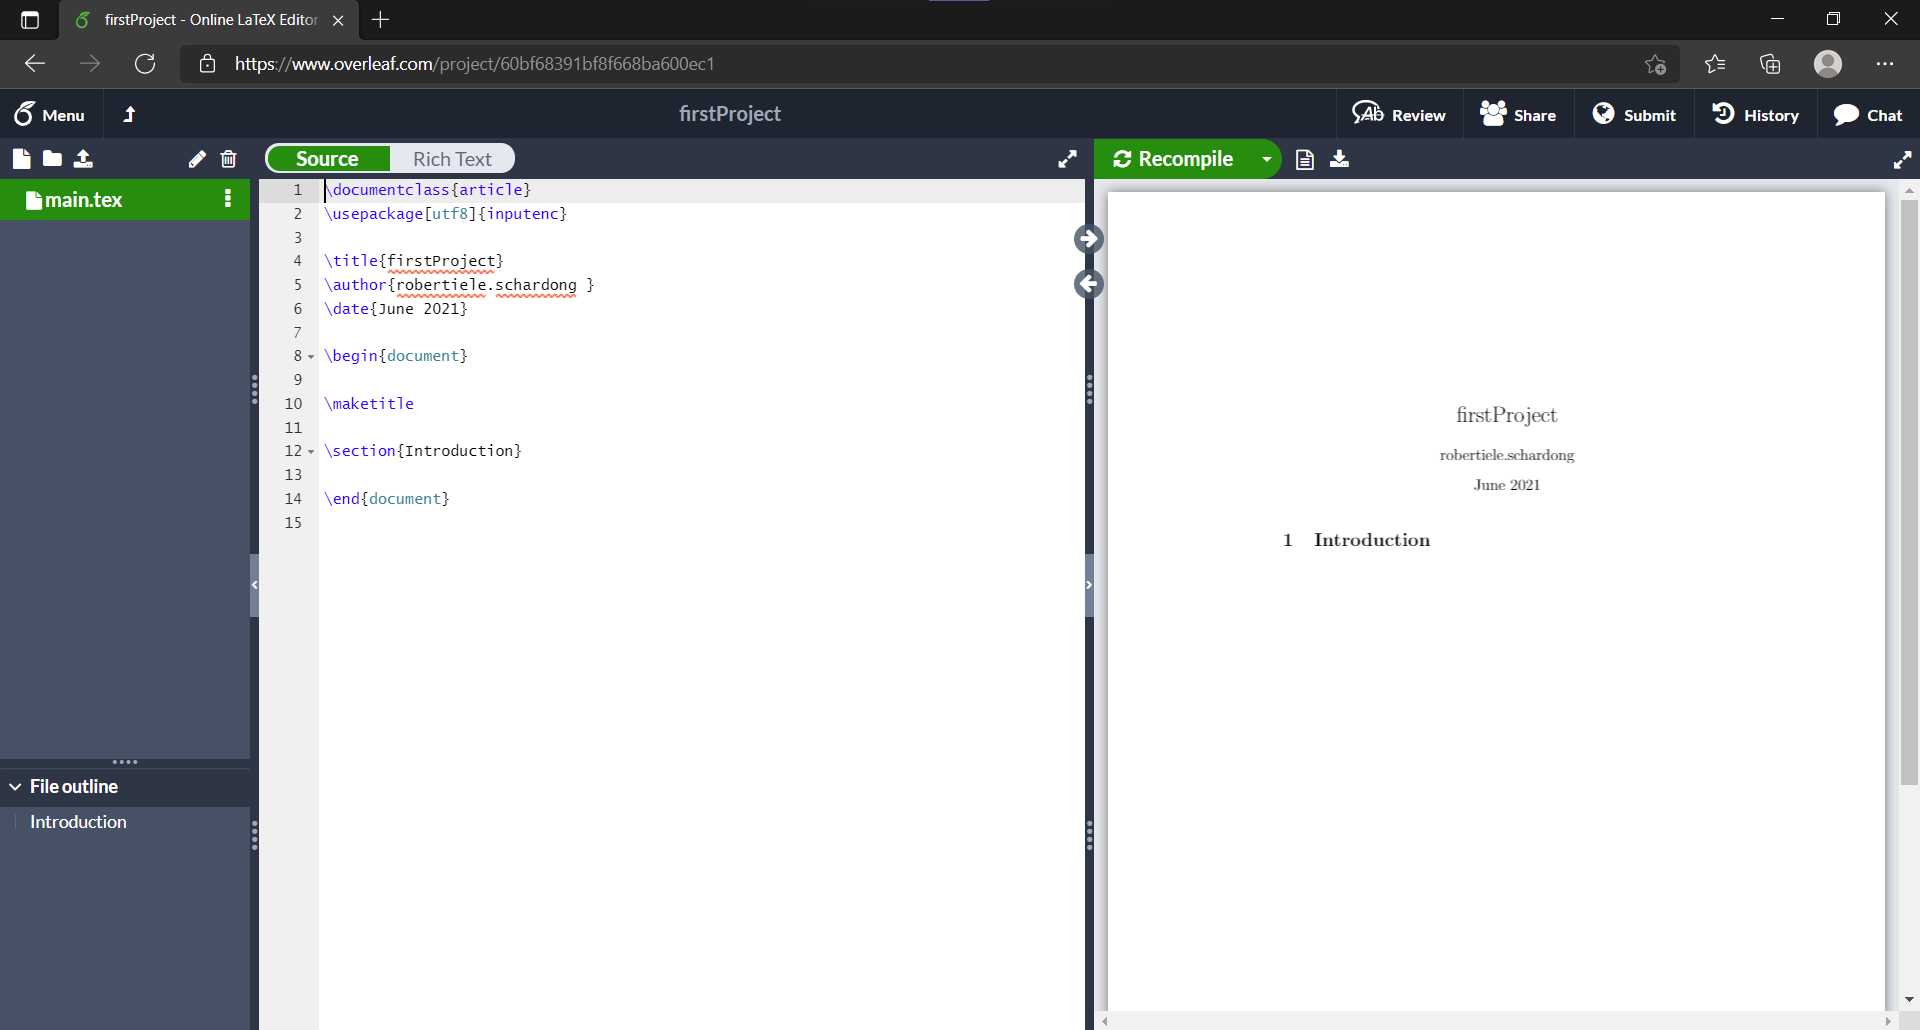
\includegraphics[width=0.8\textwidth]{../images/blankProject.png}
    \end{figure}
\end{frame}

\begin{frame}
    \frametitle{Referências}
    \nocite{overleafBeamer,overleafDocumentation,overleafTemplates}
    \printbibliography[]{}
\end{frame}
\end{document}
